\section{The Superior Places}

The order of the places\footnote{Where Dorotheus does not provide a descriptive name for a place the commonly used Greek name has been given.}, according to their \textsl{superiority} or \textsl{power} for effecting good in the person's life, relative to each other is:

\begin{description}[labelindent=0em, labelwidth=4em, labelsep=0.5em, leftmargin =!, align=right, itemsep=0em]
\item[1st] Ascendant
\item[10th] Midheaven
\item[11th] \textsl{[Good Daimon]}
\item[5th] Children
\item[7th] Marriage
\item[4th] Angle of the Earth
\item[9th] \textsl{[God]}
\item[] ------------------------
\item[3rd] Joy of the \Moon
\item[2nd] \textsl{[Gates of Hades]}
\item[8th] Death
\item[6th] \textsl{[Evil Fortune]}
\item[12th] \textsl{[Evil Daimon]}
\end{description}

The following figure shades the seven \textsl{good} places with green; the shaded red places are not as good, going from bad to worst.
\begin{figure}[H]
\centering
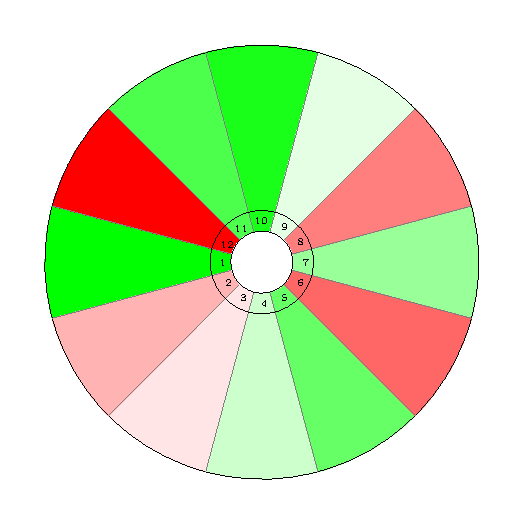
\includegraphics[width=0.7\textwidth]{diagrams/superior-places}
\vspace{-1em}
\caption{The Superior Places}
\end{figure}